\documentclass[titlepage = firstcover]{scrartcl}
\usepackage[aux]{rerunfilecheck}
\usepackage{fontspec}
\usepackage[main=ngerman, english, french]{babel}

% mehr Pakete hier
\usepackage{expl3}
\usepackage{xparse}

%Mathematik------------------------------------------------------
\usepackage{amsmath}   % unverzichtbare Mathe-Befehle
\usepackage{amssymb}   % viele Mathe-Symbole
\usepackage{mathtools} % Erweiterungen für amsmath
\usepackage[
  math-style=ISO,    % \
  bold-style=ISO,    % |
  sans-style=italic, % | ISO-Standard folgen
  nabla=upright,     % |
  partial=upright,   % /
]{unicode-math}% "Does exactly what it says on the tin."

% Laden von OTF-Mathefonts
% Ermöglich Unicode Eingabe von Zeichen: α statt \alpha

\setmathfont{Latin Modern Math}
%\setmathfont{Tex Gyre Pagella Math} % alternativ zu Latin Modern Math
\setmathfont{XITS Math}[range={scr, bfscr}]
\setmathfont{XITS Math}[range={cal, bfcal}, StylisticSet=1]

\AtBeginDocument{ % wird bei \begin{document}
  % werden sonst wieder von unicode-math überschrieben
  \RenewDocumentCommand \Re {} {\operatorname{Re}}
  \RenewDocumentCommand \Im {} {\operatorname{Im}}
}
\usepackage{mleftright}
\setlength{\delimitershortfall}{-1sp}

%Sprache----------------------------------------------------------
\usepackage{microtype}
\usepackage{xfrac}
\usepackage[autostyle]{csquotes}    % babel
\usepackage[unicode, pdfusetitle]{hyperref}
\usepackage{bookmark}
\usepackage[shortcuts]{extdash}
%Einstellungen hier, z.B. Fonts
\usepackage{booktabs} % Tabellen

%Defininierte funktionen
\DeclareMathOperator{\f}{xyz}

\ExplSyntaxOn % bequeme Syntax für Definition von Befehlen

\NewDocumentCommand \I {} {         %Befehl \I definieren,keine Argumente
  \symup{i}                         %Ergebnis von \I
} 
\NewDocumentCommand \dif {m} % m = mandatory (Pflichtargument für \dif)
{
  \mathinner{\symup{d} #1}
}

\ExplSyntaxOff % Syntax wieder ausschalten. Wichtig!

 
\subject{Versuchnummer: 803}
\title{Das Hooksche Gesetz}
\author{Marcel Kebekus \and Konstantin Mrozik}
\date{%
  Durchführung: 22.10.2019 \\
  Abgabe: 29.10.2019
  }

\begin{document}
\maketitle
\thispagestyle{empty}
\tableofcontents
\newpage

\section{Theorie}
\label{sec:Theorie}
Das Hooksche Gesetz beschreibt die elastische Verformung bei der sich die Verformung
proportinoal zur Kraft verhält.
Bei einem Federsystem führt man dabei die Federkonstante $D$ als Proportionalitätsfaktor ein.\\
Es gilt:
\\
\begin{equation}
  \vec{F}=-D \cdot \increment\vec{x} \iff D=\frac{\vec{F}}{\increment\vec{x}}
\end{equation}
\\
Das Hooksche Gesetz gilt nicht mehr, sobald die Feder überspannt wird, sie also den Bereich der
elastischen Verformung verlässt.

\section{Versuchanordnung}
\label{sec:Versuchsanordnung}

\section{Versuchsdurchführung}
\label{sec:Versuchsdurchführung}

\begin{table}
  \centering
  \caption{Messdaten}
  \label{tab:table}
  \begin{tabular}{c c c}
    \toprule
  $ x$ & $F$  & $D$  \\
    \midrule
  6  &	0.18 & 0 \\	
  12 &	0.36 & 0	\\
  18 &	0.53 & 0	\\
  24 &	0.71 & 0	\\
  30 &	0.89 & 0 \\
  36 &	1.07 & 0 \\
  42 & 	1.25 & 0 \\
  48 &	1.44 & 0 \\
  54 &	1.61 & 0 \\
  58 &	1.73 & 0 \\
  \bottomrule
\end{tabular}
\end{table}

\section{Auswertung}
\label{sec:Auswertung}


\begin{figure}
  \centering
  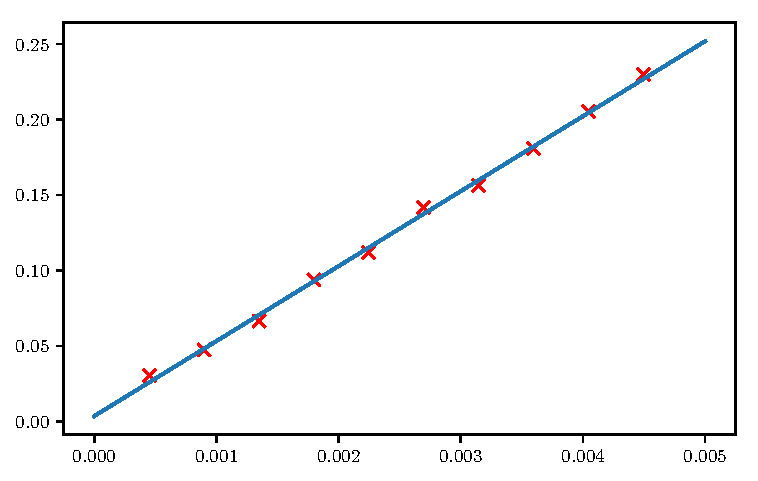
\includegraphics[width=\textwidth]{build/plot.pdf}
  \caption{Eine Beschreibung}
  \label{fig:Plot}
\end{figure}
\end{document}